\subsection{Geometry editor}
Geometry editor is used to define lines and points in two dimensional plane. These geometries are then used to define shape of the visualized simulation. Figure \ref{fig:model-geometry} describes the geometry model used by the geometry editor.

\begin{figure}[htp]
\begin{center}
  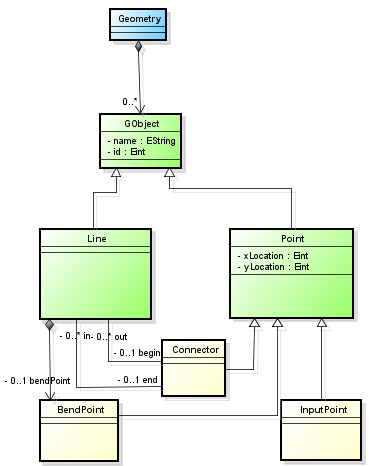
\includegraphics[width=0.8\textwidth]{image/model-geometry.png}
  \caption{Geometry domain model}
  \label{fig:model-geometry}
\end{center}
\end{figure}

\paragraph{Geometry}
The Geometry class is an abstract definition of a geometry object.

\paragraph{GObject}
The GObject is a geometry object, which can be either a line or a point. It has attributes \textbf{name} and \textbf{id}. \textbf{name} is used to name individual geometry objects, so that user can easily tell them apart. \textbf{id} is used to differentiate geometry objects from each other.

\paragraph{Point}
Point is a location in two dimensional plane. It has attributes \textbf{xLocation} and \textbf{yLocation} which refer to horizontal and vertical coordinates respectively.

\paragraph{InputPoint}
Class InputPoint is the point that petri net model place can have as geometry.

\paragraph{Connector}
Class Connector is either beginning or ending point of a line. Therefore lines that ends at the Connector are \textbf{in} and the lines that starts from Connector are \textbf{out}.

\paragraph{BendPoint}
Class BendPoint is a point used to turn lines into curved lines.

\paragraph{Line}
Class Line is a parametric curve in a two dimensional plane. The line begins at a point location \textbf{begin} and it ends at a point location \textbf{end}. \textbf{bendPoint} is a point location which defines the curve of the line, unless it doesn't have one, thus the line would be straight.
